\section{Durchführung}
\label{sec:Durchführung}
\subsection{Versuchsaufbau}
        
        Der Versuchsaufbau basiert auf einer Grundplatte, an der ein grüner Laser und ein roter Laser angebracht sind (siehe \autoref{fig:platte}). Diese sind übereinander befestigt und lassen sich auf einem Halbkreis drehen. In der Mitte dieses Halbkreises lassen sich 
        verschiedene optische Elemente befestigen. Die verschiedenen optischen Elemente sind in \autoref{fig:elemente} zu sehen.\\
        Als Schutz vor dem Laserlicht ist auf der Platte ein Reflexionsschirm angebracht. Zum Messen der verschiedenen optischen Phänomene stehen einige unterschiedliche Versuchsvorlagen zur Verfügung, die unter die Platte gelegt werden können, um die Winkel abzulesen.

        \begin{figure}[H]
            \centering
            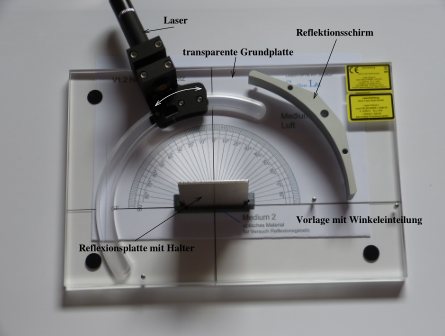
\includegraphics[width=0.5\textwidth]{images/platte.PNG}
            \caption{Die genutzte Grundplatte. \cite{400}}
            \label{fig:platte}
        \end{figure}

        \begin{figure}[H]
            \centering
            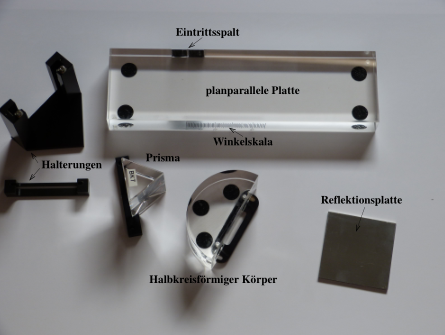
\includegraphics[width=0.5\textwidth]{images/elemente.PNG}
            \caption{Die genutzten optischen Elemente. \cite{400}}
            \label{fig:elemente}
        \end{figure}
        
        \noindent
        Bei dem Aufbau der unterschiedlichen Teil-Experimente ist darauf zu achten, dass die optischen Elemente nur an den Halterungen berührt werden, 
        da die Oberfächen durch den Fettfilm der Finger beschädigt werden können.

    \subsection{Durchführung}

        \textbf{Aufgabenteil 1}\\

            
        \noindent
            Für Aufgabenteil 1 wird ein Spiegel auf die Grundplatte gesetzt und für den grünen Laser 7 Messpaare aus Einfallswinkel und auftretendem Reflexionswinkel gemessen.
            \newline
            
            \noindent
            \textbf{Aufgabenteil 2}\\
            
            \noindent In Aufgabenteil 2 wird die planparallele Platte (siehe \autoref{fig:elemente}) aufgesetzt und es werden für den grünen Laser 7 Messpaare aus dem 
            Einfallswinkel und Brechungswinkel abgelesen. Die Platte wird so positioniert, dass man den Brechungswinkel an der planparallelen Platte ablesen kann.
            \newline
            
            \noindent
            \textbf{Aufgabenteil 3}\\

            \noindent Für Aufgabenteil 3 (Berechnung des Strahlversatzes) können die Messwerte aus Aufgabenteil 2 genutzt werden. 
            \newline
            
            \noindent
            \textbf{Aufgabenteil 4}\\

            \noindent Nun wird die planparallele Platte durch das Prisma ersetzt und die entsprechende Vorlage unter die Platte geschoben, sodass der 
            Einfallswinkel und der Ausfallswinkel aus dem Prisma abgelesen werden können. Hier werden jeweils 5 Messpaare für die beiden sichtbaren Winkel für den 
            grünen und den roten Laser aufgenommen.
            \newline
            
            \noindent
            \textbf{Aufgabenteil 5}\\

            \noindent Zuletzt werden für die Gitter mit den Gitterkonstanten 600, 300 und 100,  für rotes und grünes Licht jeweils für alle sichtbaren Beugungsordnungen auf beiden Seiten die Winkel-Abstände der Maxima zum 
            Mittelpunkt vermessen.\\